\documentclass[10pt,a4paper]{article}

\usepackage[a4paper,top=1.7cm,bottom=1.7cm,left=2.2cm,right=2.2cm,footskip=0.9cm]{geometry}
\usepackage{fontspec}
\usepackage{xeCJK}
\usepackage{graphicx}
\usepackage{booktabs}
\usepackage{tabularx}
\usepackage{array}
\usepackage[table]{xcolor}
\usepackage{titlesec}
\usepackage{enumitem}
\usepackage{caption}
\usepackage{float}
\usepackage[hidelinks]{hyperref}

% Fonts: PingFang TC for CJK, SF Pro for Latin
\setmainfont{SF Pro Text}[BoldFont={* Semibold}, ItalicFont={* Regular Italic}, BoldItalicFont={* Semibold Italic}]
\setsansfont{SF Pro Display}[BoldFont={* Semibold}]
\setCJKmainfont{PingFang.ttc}[Path=/jupyter/fonts/中文/, FontIndex=2, BoldFont=PingFang.ttc, BoldFeatures={FontIndex=10}]
\setCJKsansfont{PingFang.ttc}[Path=/jupyter/fonts/中文/, FontIndex=2, BoldFont=PingFang.ttc, BoldFeatures={FontIndex=10}]
\xeCJKsetup{CJKecglue={\hskip 0.25em plus 0.08em minus 0.04em}}
\xeCJKDeclareCharClass{Default}{"2013, "2212, "2192, "00D7}

% Spacing: 10.5pt on 17.5pt leading for body text
\renewcommand{\normalsize}{\fontsize{10.5pt}{17.5pt}\selectfont}
\renewcommand{\small}{\fontsize{9.5pt}{15pt}\selectfont}
\renewcommand{\footnotesize}{\fontsize{8.5pt}{13pt}\selectfont}
\setlength{\parindent}{0pt}
\setlength{\parskip}{5pt}

\definecolor{accent}{HTML}{2A78D6}
\definecolor{ink}{HTML}{1D1D1F}
\definecolor{muted}{HTML}{6E6E73}
\definecolor{rule}{HTML}{D2D2D7}
\definecolor{todo}{HTML}{D03B3B}

\setlist{nosep,leftmargin=1.1em,topsep=3pt,itemsep=2pt}
\setlist[itemize]{label=\textcolor{accent}{\raisebox{0.1ex}{$\bullet$}}}
\usepackage{fancyhdr}
\usepackage{lastpage}
\fancyhf{}
\renewcommand{\headrulewidth}{0pt}
\cfoot{\footnotesize\color{muted}\thepage\ / \pageref*{LastPage}}
\pagestyle{fancy}

\titleformat{\section}{\sffamily\bfseries\fontsize{13pt}{18pt}\selectfont}{\textcolor{accent}{\thesection}}{0.6em}{}
\titlespacing*{\section}{0pt}{12pt}{4pt}

\captionsetup{font={footnotesize,color=muted},labelfont={bf,color=ink},labelsep=quad,skip=5pt}
\captionsetup[table]{name=表,position=top}
\captionsetup[figure]{name=圖}
\arrayrulecolor{rule}
\renewcommand{\arraystretch}{1.15}

% ---- numbers that are still pending render in red; fill them when the runs finish ----
\newcommand{\tbd}{\textcolor{todo}{待補}}
\newcommand{\kaggle}{45.9}       % Kaggle public of result/final-notebook.csv, submitted 2026-11-15 (ref 58361835): 0.45924
\newcommand{\bestval}{46.9}       % hold-out AP of the submitted model (EMA weights, last epoch 30, 800 letterbox, no TTA): notebook 0.4688
\newcommand{\finalval}{48.2}      % hold-out AP (400 val images) of the upload setting printed by the notebook: 896 input, hflip + scales 0.75 / 1.1, one NMS: 0.4817
\newcommand{\baselineval}{12.0}   % YOLOv3 template recipe (run 001): 0.1195
\newcommand{\bestparams}{117.6M}  % parameters of the submitted model (backbone 87.6M)
\newcommand{\besttime}{6.1 h}     % training time of the submitted model in the notebook: 30 epochs, sum of the epoch times in checkpoints/final.log (resumed once after epoch 5)

\newcommand{\keynum}[2]{%
  \begin{tabular}[t]{@{}c@{}}
    {\sffamily\bfseries\fontsize{17pt}{20pt}\selectfont #1}\\[1pt]
    {\footnotesize\color{muted}#2}
  \end{tabular}}

\begin{document}
\color{ink}

{\sffamily\bfseries\fontsize{18pt}{24pt}\selectfont DL Lab 5　COCO 2017 室內 20 類物件偵測}\hfill
{\color{muted}黃毓峰　315834011}

\vspace{6pt}
{\renewcommand{\arraystretch}{1}%
\begin{tabularx}{\linewidth}{@{}*{4}{>{\centering\arraybackslash}X}@{}}
\arrayrulecolor{ink}\toprule[0.8pt]\addlinespace[6pt]
\keynum{\baselineval}{YOLOv3 範本 val AP} &
\keynum{\finalval}{上傳設定 hold-out AP，第 6 節} &
\keynum{\kaggle}{Kaggle public} &
\keynum{\bestparams}{最終模型參數量，訓練 \besttime} \\
\addlinespace[4pt]\arrayrulecolor{rule}\bottomrule
\end{tabularx}}

\section{任務與資料}
COCO 2017 的 20 個室內類別（椅子、杯子、書、刀叉等），訓練 10,193 張、驗證 3,397 張、測試 9,060 張，影像為原始 COCO 尺寸（多為 640×480）。
評分是 COCO bbox AP@[0.50:0.95]，本文的 AP 一律乘以 100。

資料有兩個特性決定了設計方向。
第一，物件小：訓練集 52,377 個框中，刀、叉、湯匙、遙控器、書、滑鼠有六到七成面積小於 32² 像素（圖 \ref{fig:cls}b），在 416 或 640 輸入下只剩幾個特徵格。
第二，類別不平衡：椅子 9,116 框、書 5,646，滑鼠只有 529；每張影像平均 5.1 個框，最多 56 個。

\section{方法}

\begin{minipage}[t]{0.50\linewidth}
\raggedright\setlength{\parskip}{5pt}
\textbf{YOLOv3 範本}　依作業要求補完 \texttt{src/yolo.py} 的 neck（三尺度各五層 1×1/3×3 卷積，上採樣串接）與 \texttt{yolo\_loss.py} 的 GIoU、focal objectness、cross-entropy 損失，以範本的 Darknet-53、416 輸入、50 epoch 訓練，val AP \baselineval（run 001）。
Anchor 配對只給每個框一個正樣本，小物件幾乎學不到。

\textbf{Anchor-free 偵測器}　最終模型全部自行實作於 \texttt{src/det\_*.py}，只用 timm 的 ImageNet-1k 分類權重。
骨幹是 ConvNeXt-B（stride 8/16/32 三層特徵），neck 是 PAFPN：先由上而下再由下而上各融合一次，每層 384 通道，融合區塊用 C2f 式的 CSP 結構。
Head 分類與回歸分開，各兩層 3×3 卷積；回歸不直接輸出座標，而是對框的上下左右四個距離各預測 16 個 bin 的離散分布（DFL），期望值即距離，單位是該層 stride。
標籤指派用 task-aligned assigner：每個真值框在中心落於框內的格子中，依 score\textsuperscript{0.5}×IoU\textsuperscript{6} 取前 10 格為正樣本，一格被多個框選到時給 IoU 最高者。
損失為對齊分數的 BCE、CIoU 與 DFL，權重 0.5 / 7.5 / 1.5。
推論用逐類別 NMS 0.65，每張最多 100 框。
\end{minipage}\hfill
\begin{minipage}[t]{0.46\linewidth}
\vspace{-6pt}
\captionof{table}{最終模型的訓練設定（016 的配方、017 的排程，在繳交的 notebook 內執行）}
\label{tab:cfg}
\small
\begin{tabularx}{\linewidth}{@{}>{\color{muted}}l >{\raggedright\arraybackslash}X@{}}
\toprule
輸入 & 800 letterbox；每 10 步整批重採樣到 480–1000（32 的倍數） \\
資料 & train + val 扣除 400 張 hold-out，共 13,190 張 \\
骨幹 & convnext\_base.fb\_in1k，drop path 0.4，梯度 checkpointing；全模型 \bestparams \\
Neck / head & PAFPN 384 通道、CSP 深度 3；DFL 16 bin \\
Optimizer & AdamW，lr 4×10\textsuperscript{−4}（骨幹 ×0.25），weight decay 0.05，batch 12，梯度裁剪 10 \\
排程 & warmup 3 epoch 後 cosine 到 10\textsuperscript{−6}，共 30 epoch（\besttime） \\
Augmentation & mosaic + 仿射縮放 0.5–1.5；copy-paste（每張貼 1–6 個其他影像的物件框）；mixup 0.15；HSV；水平翻轉；最後 10 epoch 關 mosaic \\
權重 & EMA 0.9998，取最後一個 epoch \\
\bottomrule
\end{tabularx}
\end{minipage}

\section{實驗設計}
模型選擇以驗證集 AP 為準，不用 val loss（範本以 val loss 選模型，但 001 的 val loss 第 15 epoch 起上升而 AP 到第 50 epoch 仍在升）。
各 run 固定 seed 2026，一次只改一個設定，以獨立腳本在 RTX 3090 Ti 上篩選。最終模型在 notebook 內以 train + val 從頭訓練，只留 400 張作 hold-out；沒有完整驗證集可挑 epoch，所以固定 30 epoch、取最後一輪（017：015 改 30 epoch，最後一輪 44.1 即最高點）。

\begin{table}[H]
\centering\small
\caption{各 run 的最佳 val AP（EMA 權重，不含 TTA）與小物件 AP}
\label{tab:runs}
\begin{tabularx}{\linewidth}{@{}l >{\raggedright\arraybackslash}X r r r r@{}}
\toprule
編號 & 設定（相對前一列的改動） & AP & AP\textsubscript{S} & epoch & 每 epoch \\
\midrule
001 & YOLOv3 範本：Darknet-53，416，GIoU，50 epoch & \baselineval & 2.9 & 50 & 1.3 min \\
002 & anchor-free 偵測器，ConvNeXt-T 39.9M，640，mosaic & 36.5 & – & 30 & 2.3 min \\
003 & 骨幹加 drop path 0.3 & 39.6 & – & 40 & 2.4 min \\
004 & 加 mixup 0.15 & 40.1 & – & 40 & 2.4 min \\
005 & 排程縮為 60 epoch & 40.1 & 22.9 & 45 & 2.4 min \\
006 & letterbox 640 → 800（多尺度 480–800） & 40.5 & 25.5 & 50 & 2.6 min \\
009 & 006 的骨幹換回範本的 Darknet-53（52.8M） & 38.5 & 24.6 & 40 & 3.2 min \\
007 & 006 的骨幹換 ConvNeXt-S 61.5M，drop path 0.4 & 41.4 & 26.3 & 40 & 4.6 min \\
008 & 多尺度上限 800 → 1000 & 42.0 & 26.0 & 40 & 6.1 min \\
011 & 骨幹換 ConvNeXt-B 99.8M，batch 12，排程 40 epoch & 43.0 & 26.9 & 30 & 8.4 min \\
012 & 011 改 letterbox 1024（多尺度 608–1280），batch 6 & 43.1 & 29.0 & 20 & 14.2 min \\
013 & 011 的 neck 加寬加深：384 通道、深度 3（117.6M） & 43.8 & 27.9 & 30 & 9.6 min \\
014 & 013 的骨幹換 ConvNeXt-L 226.6M，batch 6 & 43.5 & 27.7 & 20 & 16.5 min \\
015 & 013 加 copy-paste（半數 mosaic，貼 1–4 個物件） & 44.2 & 28.0 & 25 & 9.6 min \\
016 & copy-paste 每張都貼，最多 6 個 & 44.0 & 27.8 & 30 & 9.6 min \\
\midrule
最終 & 016 + 30 epoch + train+val（表 \ref{tab:cfg}）；hold-out AP & \bestval & 30.8 & 30 & 12.3 min \\
\bottomrule
\end{tabularx}
\end{table}

\section{結果}
\begin{figure}[H]
\centering
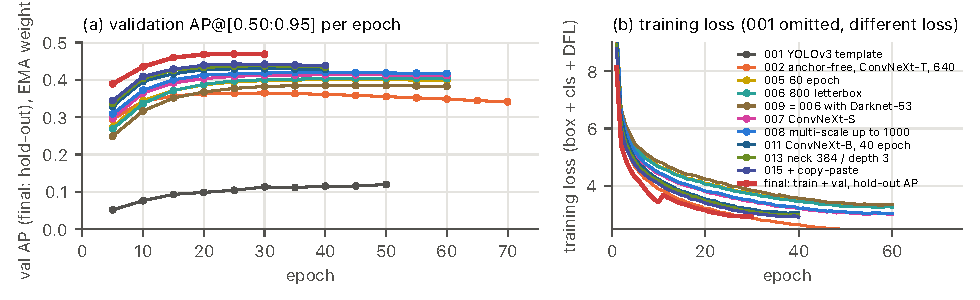
\includegraphics[width=\linewidth]{figures/curves.pdf}
\caption{(a) 每 5 epoch 以 EMA 權重算的 val AP。(b) 訓練 loss（box + cls + DFL 加權和）；001 的 loss 定義不同，不列。}
\label{fig:curves}
\end{figure}

\begin{itemize}
  \item \textbf{換掉 anchor 配對是最大的一步}：002 用參數相近的骨幹就從 \baselineval{} 到 36.5。TAL 給每個框 10 個正樣本並讓分類分數跟著 IoU 走，AP\textsubscript{S} 從 2.9 到 23 以上。
  \item \textbf{訓練資料只有 1 萬張，正則化比排程長度重要}：002 在第 30 epoch 到頂後一路下滑，訓練 loss 卻持續下降。Drop path 0.3 加 3.1 點並把高點推到第 40 epoch，mixup 再加 0.5；cosine 縮成 60 epoch 仍是 40.1。
  \item \textbf{解析度與骨幹各值 1 點上下}：800 letterbox 讓 AP\textsubscript{S} 從 22.9 到 25.5，但 AP\textsubscript{L} 掉 4.7，整體只加 0.3；訓練多尺度拉到 1000（008）補回 AP\textsubscript{L}，整體加 0.7。ConvNeXt-S 比 ConvNeXt-T 加 0.9，比 Darknet-53 加 2.9（009 同配方只有 38.5）；ConvNeXt-B 再加 1.0，且 40 epoch 就到頂。
  \item \textbf{瓶頸是過擬合，不是容量或解析度}：各 run 都在約 2.5 到 3.5 萬次更新後到頂。ConvNeXt-L（014）與 1024 輸入（012）在 24 GB 上只能 batch 6，更早到頂，只有 −0.3 與 +0.1；加寬 neck（+0.8）與 copy-paste（+0.4）才有效。最終模型因此把驗證集併入訓練：同一批 hold-out、896 單一尺度下，只用 train 的 016 是 46.1，最終模型 47.1。
\end{itemize}

\section{逐類別分析}

\begin{figure}[H]
\centering
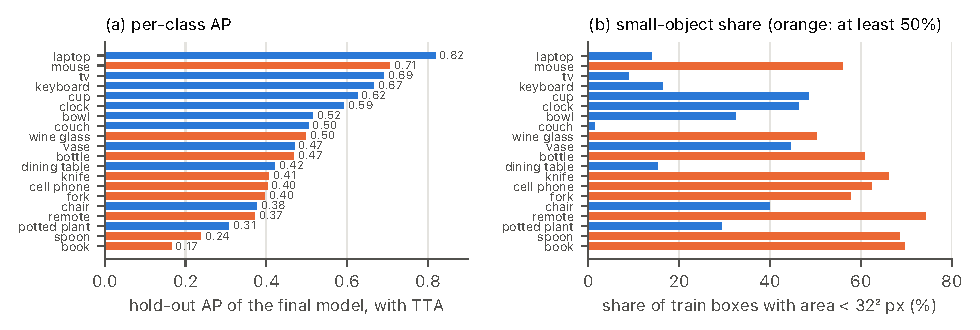
\includegraphics[width=\linewidth]{figures/per_class.pdf}
\caption{(a) 最終模型（上傳設定）在 400 張 hold-out 的逐類別 AP。(b) 訓練集各類別面積小於 32² 像素的框比例；橘色為過半的類別。}
\label{fig:cls}
\end{figure}

\begin{itemize}
  \item \textbf{弱項就是小物件類別}：書 17、湯匙 24、遙控器 37、叉 40、刀 41，小框比例都在 58\% 到 74\%；強項是筆電 82、滑鼠 71、電視 69。Hold-out 只有 400 張，單一類別的數字誤差大。
  \item \textbf{書是標註問題}：訓練框第二多，AP 卻最低：COCO 對成排的書有時逐本標、有時整排一框，高 IoU 門檻下大量被判為誤報。餐桌 42、盆栽 31、椅子 38 則難在範圍定義與遮擋。
\end{itemize}

\section{推論期的免訓練增益}

\begin{table}[H]
\centering\small
\caption{推論設定對 val AP 的影響；多尺度 TTA 把原圖、翻轉圖與各尺度縮放圖的框合併後做一次逐類別 NMS}
\label{tab:infer}
\begin{tabularx}{\linewidth}{@{}>{\raggedright\arraybackslash}X r r r@{}}
\toprule
模型與推論設定 & AP & AP\textsubscript{S} & AP\textsubscript{L} \\
\midrule
005（640 訓練），640 & 40.1 & 22.9 & 56.8 \\
005，704 單一尺度 & 40.9 & 25.0 & – \\
008（480–1000 訓練），800 & 42.0 & 26.0 & 58.5 \\
008，896 單一尺度 & 42.0 & 27.5 & 56.8 \\
016（只用 train），896 單一尺度 & 44.1 & 28.6 & – \\
016，896 + 翻轉 + 尺度 0.75 / 1.1 & 45.8 & 30.4 & – \\
\midrule
最終模型（train + val），hold-out 400 張，896 單一尺度 & 47.1 & 32.7 & 62.8 \\
最終模型，896 + 翻轉 + 尺度 0.75 / 1.1（上傳設定，Kaggle public \kaggle） & \finalval & 33.9 & 65.1 \\
\bottomrule
\end{tabularx}
\end{table}

\begin{itemize}
  \item \textbf{推論尺度可略大於訓練尺度，但不能超過訓練的最大尺度}：005（640 訓練）在 704 加 0.8，896 只剩 0.2；008 訓練到 1000 後 896 持平而 AP\textsubscript{S} 加 1.5。
  \item \textbf{多尺度 TTA 加 1.1 到 1.9 點，翻轉只加 0.3 到 0.5}：放大圖供小物件、縮小圖供大物件，AP\textsubscript{S} 與 AP\textsubscript{L} 同時上升；上傳設定的實際輸入是 672 / 896 / 992，都在訓練範圍內。
\end{itemize}

{\color{muted}\footnotesize 限制：每組設定只跑一次，0.5 點內的差異未定；hold-out 只有 400 張，與完整驗證集（3,397 張）的數字不可直接相比。}

\end{document}
